
%TODO USE BOTH SOC AND EMBEDDED?
%SOC
%Standard design techniques to secure code execution in \socs~are based on well-known cryptographic mechanisms and on (micro) architecture features to encode bus transactions~\cite{Elbaz2005}, or isolate secure code into trusted platforms~\cite{tpm_spec}, among others. Although such techniques usually provide good levels of security, most of them are either inefficient, considerably impact processor (micro) architecture design, require extensive changes in the programming tool-chain~\cite{Suh2003a}, or are so complex \cite{Suh2005} that may create unexpected security loopholes. Any solution up to this challenge should be able to use more than incremental approaches which try to re-use current cryptographic mechanisms to fill in security holes; the new generation of \iot~\soc~devices will require novel solutions which deeply integrate hardware-intrinsic security features to program execution, across the whole architecture and software stacks.
%PUF
%\textit{Physical Unclonable Functions} (\pufs) are devices which exploit the statistical distribution of hardware-intrinsic physical parameters to design functions capable of (uniquely) mapping a set of inputs (\textit{challenges}) to outputs (\textit{responses}) \cite{PRTG02}. Built upon PUF theoretical models, several constructions of essential cryptographic primitives have been proposed, mainly to support key exchange~\cite{LLG05,STO05,BFSK11}, device authentication~\cite{Suh2007}, intellectual property protection~\cite{GKST07}, oblivious transfer~\cite{R10,BFSK11} and commitment schemes~\cite{BFSK11}. The myriad of cryptographic primitives which could benefit from \pufs~has driven the search for efficient real-world implementation of these devices.
%Although silicon \pufs~have gained a lot of attention, they are still under strong scrutiny, as they can undergo a number of attacks like: (1) reverse engineering \cite{Nedospasov2013}, (2) characterization of the physical parameters \cite{Tajik2014}, (3) modeling \cite{Becker2015}, and (4) emulation \cite{Helfmeier2013}. Even though there are still many concerns about the overall security of \pufs, their simplicity, low-power consumption and speed are very attractive design features for some application domains~\cite{1502786} (e.g. \iot~devices). One of the potential applications of \pufs~in \iot~devices would enable integrity checking and authentication of program code and data. Yet very few works have addressed that using \pufs\cite{Suh2005}. Thus additional research needs to be done in order not only to improve \puf~security, but also to allow its integration into processor architecture and software stacks.

%Recently, \textit{Computer Security by Hardware-Intrinsic Authentication} (\system) was presented in~\cite{Hoffman2015}. \system~proposes a new secure program execution model which employs a new \puf-based authentication mechanism aimed at ensuring code and data authenticity for a given program\slash{}processor pair. Specifically, the system generates an authentication tag (called \ptag) to every instruction and data cache line at the very first moment that it runs in the processor. This authentication tag is later verified for integrity, ensuring that program instructions and data are not violated in runtime, and thus programs will execute correctly during the lifetime of the device. 
%This work  intents to extend the preliminary contributions in \cite{Hoffman2015}. In particular, design a \cshia~\fpga~prototype in conjunction with a security analysis and further evaluate its impact on performance and robustness .

%Embedded systems
The demand for code/data integrity and authenticity has steadily increased. The broad spectrum of known attacks currently poses a threat to a variety of embedded systems that need constant protection against tampering. An excellent example of such systems are the ones that are equipped with large external non-volatile memories to store software and data, like voting machines, smart metering devices and employee attendance control systems. These systems need to provide integrity and authenticity, but usually not secrecy or confidentiality, in order to be easily audited by governmental authorities and independent experts.

Due to the stringent nature in available resources of embedded systems, software solutions for code and data integrity do not lead to efficient solution due to their impact in the performance and power consumption of the system. Besides, software authenticity could involve a third-party certification authority, considerably increasing the complexity of the final solution, thus making hardware a potentially effective solution to such a problem. A myriad of hardware solutions for code and data authenticity and integrity have been proposed in the literature (\cite{Suh2005:AEGISImplementation,Vaslin2009:OTP,Hong2010:FEDTIC,Bobade2015:SecurityFPGA}), however, some of these solutions target high-end embedded systems or more robust configurations.
%(guido is rigth this is  not mentioned anywhere else)requiring at least a two-level cache in the processor for their performance overhead not to be prohibitive.
Other approaches need modifications on the Instruction Set Architecture (\isa) or processor datapath, leading to complete redesign of code, compilers, operating systems, among others. Moreover, not all solutions provide integrity and authenticity.

Recently, an architecture aiming at code/data authenticity and integrity was proposed in \cite{Hoffman2015}. The Computer Security by Hardware-Intrinsic Authentication (\cshia) provides authenticity by authenticating all memory blocks of the external memory using a unique key extracted from Physical Unclonable Functions (\pufs) implemented in each instance. The authentication tags (called \ptags) are computed during an enrollment procedure and later verified or updated on runtime for each memory block brought to the processor. The main advantages of \cshia~ over the previous hardware solutions are that it does not require changes in the \isa~or datapath, being adaptable to most of the embedded system architectures while providing complete software compatibility, it also uses a separate bus for the tag memory, which gives designers the freedom to match timing requirements so as to hide verification overhead.
\mario{Add: \\  the research proposal of this dissertation , goals of the msc and the contributions , not necessarily in  subsections maybe add research questions }

%TODO  Focus on the architecture  and design tradoffs, caio is going to describe the security part 

%, we evaluated performance and storage overheads, computed area and power estimates, and also performed a security analysis. 
%The \cshia~implementation enables two solutions against replay attacks: timestamps or \mt. To the best of our knowledge, it is the first time that both solutions are evaluated in the same architecture. The results showed that the \cshia's timestamp instance is the best one, when taking into account performance degradation, area and energy overhead. It presented only 2.76 \% of performance penalty on average, while the \mt~instance showed an average 5.77 \% reduction on performance.




\section{Contributions}
\label{sec:contributions}
The main contributions to this work are the following: 
\begin{enumerate}[label=(\alph*)]
    \item it provides the first hardware implementation of the CSHIA architecture ,using LEON3 processor;
    \item it analyses the trade-offs of the resulting architecture \mario{Expand  what will be shown , are power ?? }
\end{enumerate}

% the publications submitted will be mentioned  inthe conlcusions and in te presentation
% \section{Publications}
% \label{sec:publications}
% The contributions of this work were published  in the following venues 
% \begin{itemize}
% \item{Pub0} Publication 1  - description 1
% \item{Pub1} Publication 2 - description 2
% \end{itemize}

\section{Organization of the dissertation}
\label{sec:organization_of_dissertation}
This work is organized as follows. Chapter \ref{chap:fundamental_concepts} introduces the necessary concepts  needed for this work. A review of the related work is presented in the chapter \ref{chap:related_work}.  The CSHIA architecture implementation is described in Chapter \ref{chap:cshia_architecture}. Chapter \ref{chap:cshia_prototype} details the prototype and all implementation requirements. The evaluation of the prototype is presented in Chapter \ref{chap:cshia:evaluation} ans Chapter \ref{chap:conclusion} concludes this work.
\begin{figure*}[!ht]
	\centering
	\includegraphics[scale=0.42]{organi}
% 	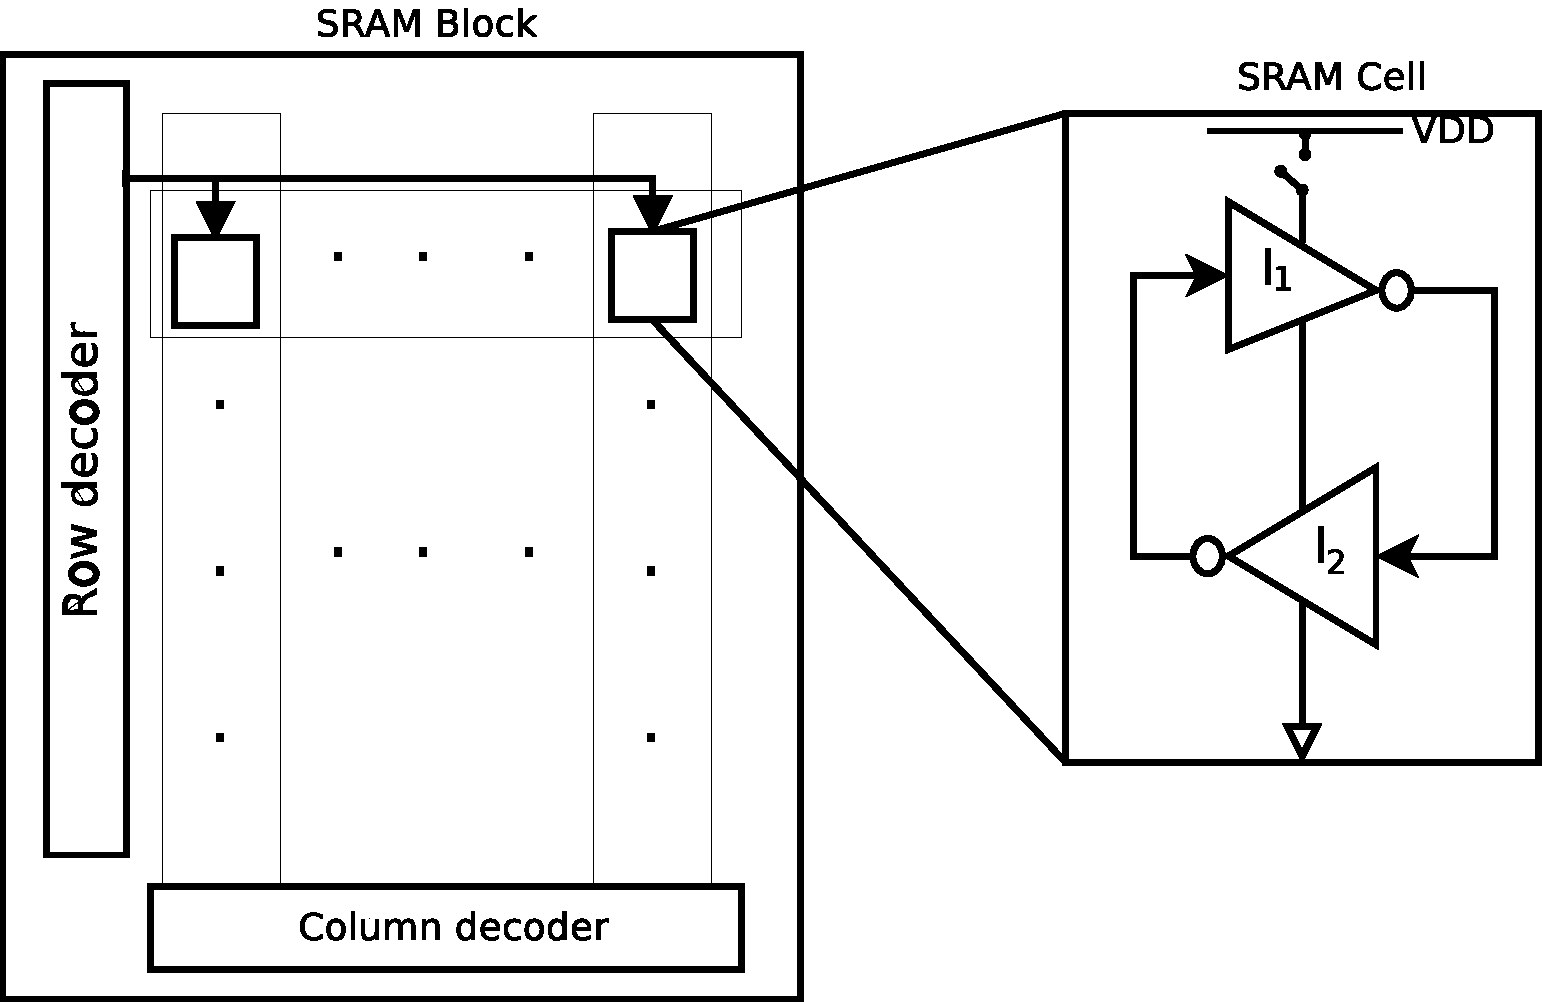
\includegraphics[width=\textwidth]{figures/pdf/spuf}
	\caption{Visual organization of the dissertation.}
%	\vspace*{-9pt} 
	\label{fig:spufexample}
\end{figure*}

%Security issues in embedded system are discussed in Section \ref{sec:Security-Issues-in-Embedded-Systems}. Section \ref{sec:CSHIA} describes the architecture. Section \ref{sec:Implementation} provides details about the implementation of \cshia~in the \leon's platform. Section \ref{sec:Experiments-and-Results} discusses experiments and results. A security analysis of the \cshia~implementation is presented in Section \ref{sec:Security-Analysis}. Section \ref{sec:Related-Work} discusses related work and Section \ref{sec:Conclusions} concludes this work.

